\section{Case-study }\label{sec:case-study}

Next, we present a case study for systematically applying the distributed self-adjusting systems architecture to a common but notoriously difficult problem: software packet classification \cite{gupta2001algorithms}. The \emph{goal} is to demonstrate the general engineering methodology by assembling \emph{existing} techniques into a distributed self-adjusting scheme and understand when, and to what extent, superlinear scaling emerges. We consider it a success of we find at least one synthetic and one realistic workload that produces positive result (as we will see, we find way more). It is a stated \emph{nongoal} to conceive novel algorithms and present new capabilities, let alone to present the fastest ever software packet classifier implementation. % (that award undeniably goes to DPDK \texttt{rte\_acl} \cite{rte-acl})
Still, our multicore self-adjusting firewall will prove several times faster than the default Linux kernel implementation on a wide range of workloads.

Recall, to achieve superlinear scaling we have to combine a locality-boosting load balancer with a self-adjusting algorithm. There is a broad range of potential use cases that come with an adequate self-adjusting algorithm \cite{SleatorT85Splay, BentleyCL93, HesterH85, HesterH85, BentleySTW86, Avin0020, ParkM12}. Eventually, we stayed with packet classification for the following reasons. First, packet classifiers possess an intrinsic linear lookup structure, where the administrator can define chains of rules that must each be matched in the order of priority for each packet. This makes packet classification an appealing candidate for applying the move-to-front heuristics (but see ramifications below). Second, the default Linux firewall implementation, \nftables, uses a static list of rules ordered priority-wise and performs linear a linear sweep of the rule chain for each packet. This will buy us the non-self-adjusting baseline for free. Third, there is an infamously difficult theoretical problem underlying packet classification \cite{10.1145/2619239.2626294,10.1006/jagm.1996.0063} so that it has so far resisted any effort for finding a provably polynomial time algorithm (in terms of rule-width and size) \cite{PacutVAPRS2022, 10.1145/2619239.2626294, 10.1145/1851182.1851208, 10.1145/863955.863980, gupta2001algorithms}. This is so much so that many existing implementations \cite{Srinivasan1999,188960} are susceptible to a denial-of-service attack that exploits the vast algorithmic complexity \cite{10.1145/3359989.3365431}. Fourth, the Linux kernel network stack offers several flexible software and hardware based load balancers for dispatching jobs to multiple parallel classifier instances running on different CPU cores \cite{rss-linux}. These readily support 5-tuple hashing but also many other policies for obtaining a hash on the packet header fields, and we can easily reuse these to implement the locality boosting load balancer component. And fifth, there is a geneal self-adjusting algorithm recently published in the literature that lends itself to be implemented in \nftables for experimentally checking superlinear scaling right on the Linux kernel firewall \cite{10228937}.

\subsection{Self-adjusting packet classification}
\label{sec:sa-pack-class}

We take off from the default \texttt{nftables} firewall implementation in the Linux kernel and 

\begin{table}[t]
  \centering
  \begin{small}
    \renewcommand{\tabcolsep}{2pt}
    \begin{tabular}{r|l|l|r|r|l}
      \textbf{Prio} & \textbf{Proto} & \textbf{Src IP} & \textbf{Dst IP} & \textbf{Dst Port} & \textbf{Action}\\
      \hline
      1 & UDP & 192.168.178.33 & 23.0.0.45 & 53 & ACCEPT\\
      2 & TCP & 10.10.10.0/24 & 23.0.0.45 & 443 & DROP\\
      3 & TCP & 10.10.10.10/32 & 23.0.0.45 & ANY & ACCEPT\\
      4 & UDP & 192.168.178.0/24 & 23.0.0.45 & 53 & DROP\\
      5 & IP & 192.168.0.0/16 & 23.0.0.0/8 &  & ACCEPT\\
    \end{tabular}
  \end{small}%
  \caption{Sample firewall rule set}
  \label{fig:class-sample}
\end{table}

\begin{figure}[t]
  \centering
  \begin{small}
    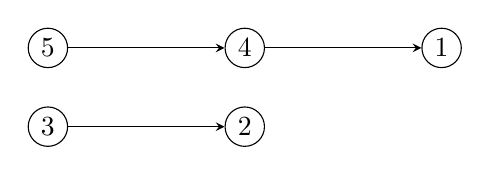
\begin{tikzpicture}[->,>=stealth,node distance=2.5cm, auto, every node/.style={circle,draw,minimum size=0.5cm,inner sep=2pt}]
      % Branch 1
      \node[circle,draw] (5) {5};
      \node[circle,draw,right of=5] (4) {4};
      \node[circle,draw,right of=4] (1) {1};
      
      % Branch 2
      \node[circle,draw,below of=5,yshift = 1.5cm] (3) {3};
      \node[circle,draw,right of=3] (2) {2};
      
      % Edges
      \draw (5) -- (4);
      \draw (4) -- (1);
      \draw (3) -- (2);
    \end{tikzpicture}
  \end{small}
  \caption{Dependency graph}%
  \label{fig:class-dep}
\end{figure}

\begin{algorithm}
  \caption{Move Recursively Forward (MRF)}
  \label{alg:alg}
  \begin{small}
    \begin{algorithmic}[1]
      \Procedure{MRF}{$y$}
      \If{$y$ has no dependencies}
      \State Move $y$ to the front of the list
      \Else
      \State Let $z$ be the direct dependency of $y$
      \State Move node $y$ to position$(z) + 1$
      \State \Call{MRF}{$z$}
      \EndIf
      \EndProcedure
    \end{algorithmic}
  \end{small}
\end{algorithm}

\subsection{Locality boosting with RSS}
\label{sec:sa-rss}




\subsection{Implementation}
\label{sec:sa-nf-tables-impl}
In our case study, we focus on the \textit{nf\_tables} firewall within the Linux Kernel. First, we replace the static list used to store the rules with the self-adjusting RMF list. 
In order to achieve optimal scaling properties and avoid any lock contention, the ruleset is replicated for all CPUs. To distribute the network traffic across all cores, we use RSS hash filter options (\textit{rx-flow-hash}).
This generates a hash using the header fields within the network packet, which then dictates to which receive queue the packet is delivered.
We use Classbench \cite{4237157} to generate the rulesets and traffic traces with which we test our implementation using real-world resembling scenarios. 


\subsection{Evaluation}
\label{sec:sa-nf-tables-eval}

- synthetic microbenchmarks and realistic macrobenchmark: rulesets and traffic

% when superlinear scaling appears
\noindent%
\textbf{Superlinear scaling.} %  (3 figs + 1 with Jonas's stats?)
\begin{itemize}
\item no dependency rule-set and uniform traffic
\item rule-template: 1.2.3.4+udp-dst:i[1,n], where n is a parameter: 997, 4999, 10007 (primes)
\item flows: uniform + zipf: 20000 * packets=pcap
\item RSS: 5-tuple hash
\item one fig per rule size (packet rate): 4 plots: SA+uniform, SA+zipf, baseline+uniform,baseline+zipf
\item takeaway: rule size + traffic-locality do not matter (3 figs + 1 with Jonas's stats?)
\end{itemize}

% when superlinear scaling deteriorates into linear because SA does not work
\noindent%
\textbf{Active flow size.} %  (1 fig)
\begin{itemize}
\item same no-dep rule-set (udp-dst) + 5, 50, 500 flows per rule
\item RSS: 5-tuple hash
\item fig: 3 scaling laws, one for each active-flow-size: speedup (speedup: normalized for the single-core rate)
\item takeaway: the more the flow count the more rules are replicated across cores and the larger the working set size and superlinearity vanishes
\end{itemize}

\noindent%
\textbf{Rule dependencies.} % (1 fig)
\begin{itemize}
\item rule template: 1.2.3.4/{32,28,24,20,16,12,8,4,0}+udp-dst:i[1,500]
\item   traffic template: uniform: 1.2.3.4:i (500 flows) 
\item   3 rules-sets: small-dep (/0 and /32 for each chain), medium-dep (/{32,24,16,8,0}  for each chain), high-dep (/{32,28,24,20,16,12,8,4,0}  for each chain)
\item   RSS: 5-tuple hash
\item: fig: 3 scaling laws: speedup (normalized for the single-core rate)
\item takewaway: the more dependencies, the less superlinearity (dependencies must be in the working set at each thread)
\end{itemize}

\noindent%
\textbf{Locality boosting.} % (1 fig)
\begin{itemize}
\item benchmark the high-dep rule-set with different RSS hashes: bad hash: IP-dst(everything goes to 1 cpu, no scaling), 5-tuple hash (same as in the previous case), good hash: udp-dst hash (dep chains are partitioned across cpus: only a few chains per each CPU) 
\item  takeaway: load-balancing policy matters, the less locality-boosting, the less superlinearity
\end{itemize}

% realistic macrobenchmark
\noindent%
\textbf{Real workload.} % (3 figs)
classbench: the good news (3 figs with 3 different seeds + 5000 rules) + throughput and latency diagrams

%%% Local Variables:
%%% mode: latex
%%% TeX-master: "distributed_mrf"
%%% End:

